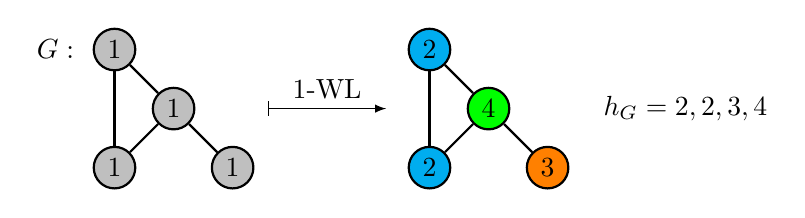
\begin{tikzpicture}
    \tikzset{line/.style={draw,thick}}
    \tikzset{arrow/.style={line,->,>=stealth}}
    \tikzset{node/.style={circle,inner sep=0pt,minimum width=15pt}}
    
    \draw (-1.5,0.75) node {$G:$};
    \node[line,node,fill=lightgray] (x1) at (-0.75, 0.75) {1};
    \node[line,node,fill=lightgray] (x2) at (-0.75, -0.75) {1};
    \node[line,node,fill=lightgray] (x3) at (0.75, -0.75) {1};
    \node[line,node,fill=lightgray] (x4) at (0, 0) {1};
    
    \path[line] (x1) to (x2);
    \path[line] (x1) to (x4);
    \path[line] (x2) to (x4);
    \path[line] (x3) to (x4);

    \draw [|-latex] (1.2,0) -- node [text width=2.5cm,midway,above,align=center ] {1-WL} (2.7,0);
    

    \node[line,node,fill=cyan] (x1) at (-0.75 + 4.0, 0.75) {2};
    \node[line,node,fill=cyan] (x2) at (-0.75 + 4.0, -0.75) {2};
    \node[line,node,fill=orange] (x3) at (0.75 + 4.0, -0.75) {3};
    \node[line,node,fill=green] (x4) at (0 + 4.0, 0) {4};
    
    \path[line] (x1) to (x2);
    \path[line] (x1) to (x4);
    \path[line] (x2) to (x4);
    \path[line] (x3) to (x4);

    \draw (6.5, 0.0) node {$h_G = \MSopen 2, 2, 3, 4 \MSclose$};

    
    
    \end{tikzpicture}
